\documentclass{article}
\usepackage{amsmath}
\usepackage{fullpage}
\usepackage{graphics}
\usepackage{graphicx}

%www.texample.net
\usepackage{tikz}
\usetikzlibrary{shapes,arrows}

\begin{document}

\tikzstyle{cond} = [diamond, draw, fill=blue!20, text width = 4.5em,
                    text badly centered, node distance=3cm, inner sep = 0pt]
\tikzstyle{block}= [rectangle, draw, fill=blue!20, text width = 10em,
                    text centered, minimum height = 2em]
\tikzstyle{line} = [draw, -latex']
\tikzstyle{term} = [draw, rectangle, rounded corners, fill=red!20,
                    node distance=3cm, minimum height = 2em]

\title{IPOL - CLG Optical Flow}
\author{Jorge Jara, Jos{\'e} Delpiano \& Steffen H{\"a}rtel,\\
SCIAN-Lab, DCC, Biomedical Neuroscience Institute, University of the Andes,\\
University of Chile}
\maketitle

\section{Overview}
Optical flow (OF) approaches calculate vector fields which determine the 
apparent velocities of objects in time varying image sequences. OF was introduced 
in 1981 by Horn and Schunck (HS) as ``...the distribution of apparent velocities 
of movement of brightness patterns in an image'' \cite{HS81}. The idea contains 
two basic assumptions: ``brightness value constancy'' and ``smooth flow of the 
intensity values'' between two successive images. At about the same time, Lucas 
and Kanade (LK) presented a method for motion estimation between images, 
considering constant motion patterns for image patches \cite{LK81}. While the HS 
model is intended to solve the problem for a non-null motion field over the 
entire image -a \textit{global} approach- the LK model can produce homogeneus 
piece-wise motion field ``patches'' -as a \textit{local} approach- allowing null 
motion regions. Several variations of the original HS- and LK-OF approaches have 
been published. The presented algorithm is known as the combined local global 
(CLG) method of Bruhn et al. \cite{Bruhn02}, encompassing properties of both the 
global HS- and the local LK-OF models. The CLG-OF aims to improve the accuracy 
of the OF field for small-scale variations while retaining the HS-OF benefits of 
dense and smooth vector fields.


An online implementation of this algorithm is available for 2D images, using the 
numerical scheme proposed in \cite{Bruhn05rt}. It must be noted that the 
algorithm works on grey-scale images. Color images will be converted to single 
channel (grey-scale) prior to the online OF computation.


\section{Description}

\subsection{Horn-Schunck Global Approach}

The HS model assumes ``brightness constancy'' and a ``smooth flow'' pattern 
between two consecutive images. Let $I = I(x,y,t)$, the constancy assumption 
is expressed as $\partial I / \partial t = 0$. Let $\underline{V}$ the optical 
flow vector field, $\underline{V} = [u(x,y,t),v(x,y,t),1]^T$. The HS-OF is 
defined from a first-order Taylor expansion
\begin{align}
I(x+u, y+v, t + \Delta t) - I(x, y, t) = 0 \implies I_x u + I_y v  + I_t = 0
\end{align}

Integrating over the image domain $\Omega$, an ``energy functional'' is defined
as

\begin{align}
E_{HS}(\underline{V}) = \int_{\Omega}(I_xu+I_yv+I_t)^2
                                      + \alpha(|\nabla u|^2+|\nabla v|^2)dxdy
\end{align}

The \textbf{global regularization coefficient} $\alpha > 0$ is a smoothing factor 
for the OF field. Higher values produce more homogeneus fields, while lower 
values allow more variating displacement vectors in a given image region. It must 
be noted that this coefficient is denoted by $\alpha^2$ in the HS-OF article 
\cite{HS81}, instead of $\alpha$ in the CLG-OF article \cite{Bruhn02}.


\subsection{Lucas-Kanade Local Approach}

The LK approach assumes that the flow is constant in a neighbourhood of size 
$\rho$, computing the optical flow for all the pixels in that neighbourhood, 
by the least squares criterion

\begin{align}
E_{LK}(u,v)=K_{\rho} * (I_x u + I_y v + I_t)^2
\end{align}

A minimum $(u,v)$ for $E_{LK}$ satisfying $\partial_uE_{LK} = 0$ and 
$\partial_vE_{LK} = 0$ yields the following system of equations

\begin{align}
  \left[
    \begin{matrix}
      K_\rho * (I_x^2)   & K_\rho * (I_x I_y) \\
      K_\rho * (I_x I_y) & K_\rho * (I_y^2) \\
    \end{matrix}
  \right]
  \left[
    \begin{matrix}
      u \\
      v \\
    \end{matrix}
  \right]
=
  \left[
    \begin{matrix}
      - K_\rho * (I_x I_t) \\
      - K_\rho * (I_y I_t) \\
    \end{matrix}
  \right]
\end{align}

If the image gradients are not zero, the matrix for the system is invertible 
and a solution can be computed.


\subsection{Bruhn et al. Combined Local-Global Approach}

Bruhn et al. \cite{Bruhn02} defined the CLG-OF by an integral functional 
that encompasses both the HS and the LK approaches. This combined approach 
aims to produce dense flow fields (characteristic of the global methods) which 
are robust against noise, by employing smoothing terms based on both the global 
and local approaches.

Let
\[ \nabla_3I = [I_x, I_y, I_t]^T \]

The HS-OF energy functional can be written as
\begin{align}
 E_{HS}(\underline{V}) = \int_{\Omega}
                          (\underline{V}^T (\nabla_3I \nabla_3I^T) \underline{V}
                         + \alpha(|\nabla u|^2+|\nabla v|^2)) dx dy
\end{align}

The CLG-OF energy functional introduces a smoothing term in $\nabla_3I$. The 
corresponding energy functional is defined as

\begin{align}
 E_{CLG}(\underline{V}) = \int_{\Omega}
                          (\underline{V}^T J_\rho(\nabla_3I)\underline{V}
                         + \alpha(|\nabla u|^2+|\nabla v|^2)) dx dy
\end{align}

with
\[ J_\rho(\nabla_3I) = G_\rho \otimes (\nabla_3I \nabla_3I^T) \]

$J_\rho$ acts as a \textbf{local spatio-temporal derivative smoothing} term, 
defined as a convolution $\otimes$ between a bi-dimensional Gaussian kernel 
$G_\rho$, with standard deviation $\rho$, with the matrix 
$(\nabla_3I \nabla_3I^T)$. If $\rho = 0$ no local smoothing occurs, making the 
CLG-OF functional equal to the HS-OF. If $\alpha = 0$ the functional becomes 
equivalent to the LK-OF model.

\label{numericalSolution}
\subsubsection{Numerical solution}

The minimum of the energy functional has to satisfy the Euler-Lagrange equation, 
in the form of a system of partial differential equations

\begin{align}
 \alpha \Delta u - (J_{11}u + J_{12}v + J_{13}) = 0 \\
 \alpha \Delta v - (J_{21}v + J_{22}v + J_{23}) = 0
\end{align}

with $J_{ik}$ denoting the elements of the matrix $J_\rho$. Neumann boundary 
conditions are assumed, given by

\begin{align}
 \partial_n u = 0, \partial_n v = 0
\label{eqn:NeumannBC}
\end{align}

Although the CLG-OF can be equivalent to the HS-OF depending on the parameter 
values, different discretization schemes were used for both models in their original 
versions. This can lead to slightly different results when both methods are applied 
to the same set of images (see for example \cite{Delpiano11,Hubeny07} 
which evaluate OF for fluorescent objects in microscopy images).\\

The discrete derivatives in space and time (used to compute $J_\rho$) are 
computed as

\begin{align}
 I_x \approx I \otimes \frac{1}{12h} [ 1 \ -8 \ 0 \ 8 \ -1 ]_x |_{x_i,y_j,t_k} \\
 I_y \approx I \otimes \frac{1}{12h} [ 1 \ -8 \ 0 \ 8 \ -1 ]_y |_{x_i,y_j,t_k} \\
 I_t \approx I(x_i, y_j, t_{k+1}) - I(x_i, y_j, t_k)
\end{align}

where $h$ is a step size of the discretized domain (a single pixel can be taken 
as $h=1$, for instance, and $A_l |_{x_i,y_j,t_k}$ denotes the mask vector $A$ 
applied in the $l$ axis at image position $(x_i,y_j,t_k)$ (the central element 
of the mask corresponds to the image pixel $(x_i,y_j,t_k)$).\\

$J_\rho$ is computed as follows: (i) $J_0 = \nabla_3I \nabla_3I^T$ is computed, 
(ii) if $\rho = 0$ then $J_\rho = J_0$, otherwise (iii) a square gaussian matrix 
$G_\rho$ is defined with standard deviation $\rho$, and (iv) 
$J_\rho = J_0 \otimes G_\rho$.\\

The laplacian is computed by a convolution between the OF components and a kernel 
matrix $M$ as

\begin{align}
 \Delta u_{x_i, y_j, t_k} \approx U \otimes M |_{x_i, y_j, t_k}
 \Delta v_{x_i, y_j, t_k} \approx V \otimes M |_{x_i, y_j, t_k}
\end{align}

with
\[
 M = \left[ \begin{matrix}
  0 &  1 & 0 \\
  1 & -4 & 1 \\
  0 &  1 & 0
 \end{matrix} \right]
\]


\subsection{Iterative scheme}

The first step in the CLG-OF computation is a gaussian smoothing (optional) of 
the input images. Upon the result, the numerical solution is computed using a 
Gauss-Seidel iterative scheme, according to \cite{Bruhn05rt}. Given the system 
$Ax = b$, the matrix $A$ is decomposed in the form $A=D-L-U$, with $L$ a 
diagonal matrix and $L,U$ lower and upper triangular matrices. Then, the $k$-th 
Gauss-Seidel iteration for $x$ is given by $x^{k+1}=(D-L)^{-1}(Ux^k+b)$. From a 
given initial value $x^0$, the equation is solved iteratively until a convergence 
criterion is reached. In this case, two equations must be solved for the OF field 
components, $(u,v)$ as described next. For these equations the subscript notation 
is changed from two indexes (e.g. $u_{ij}$) to one index ($u_i$), in order to be 
consistent with the original article.\\

Let $U$ and $V$ the matrices storing the $x$ and $y$ components of the OF field 
at a given position $i$ and iteration $k$, the values of the OF field ($u_i$, 
$v_i$) for the next iteration are computed as

\begin{align}
 u_i^{k+1} = \frac{\displaystyle \sum_{l=1}^{2}
                     \frac{\alpha}{h_l^2} \left( \sum_{j \in N_l^-(i)} u_j^{k+1}
                                         + \sum_{j \in N_l^+(i)} u_j^{k} \right)
                                              - (J_{12i} v_{i}^k + J_{13i})}
                  {\displaystyle \sum_{l=1}^{2} \frac{\alpha}{h_l^2} |N_l(i)| + J_{11i}} \\
 v_i^{k+1} = \frac{\displaystyle \sum_{l=1}^{2}
                     \frac{\alpha}{h_l^2} \left( \sum_{j \in N_l^-(i)} v_j^{k+1}
                                         + \sum_{j \in N_l^+(i)} v_j^{k} \right)
                                               - (J_{21i} u_{i}^{k+1} + J_{23i})}
                  {\displaystyle \sum_{l=1}^{2} \frac{\alpha}{h_l^2} |N_l(i)| + J_{22i}}
% Note: there is an error in the original article Bruh05rt in 2nd eq, last term
% in the numerator, it is J_{23i} instead of J_{13i}
\end{align}

where $N_l(i)$ denotes the neighbors of pixel $i$ in direction of axis $l$ 
belonging to $\Omega$, making

\[ N_l^+(i) = \left\{ j \in N_l(i) | j > i \right\} \]
\[ N_l^-(i) = \left\{ j \in N_l(i) | j < i \right\} \]

At this point, a variant of the Gauss-Seidel method is used. The so-called 
\textit{pointwise coupled Gauss-Seidel} scheme update the OF values for each 
pixel synchronously \cite{Bruhn05rt,Hac93}. Let the vector 
$w_i^{k+1} = (u_i^{k+1}, v_i^{k+1})$ at pixel $i$, the iteration becomes 

\begin{align}
 w_i^{k+1} = M_i^{-1} g_i^{k+1/2}
\label{eqn:pcGaussSeidel}
\end{align}

with
\[ M_i =
 \left[ \begin{matrix}
  \displaystyle \sum_{l=1}^2 \frac{\alpha}{h_l^2} \left| N_l(i) \right| + J_{11i} &  J_{12i} \\
  J_{21i}  & \displaystyle \sum_{l=1}^2 \frac{\alpha}{h_l^2} \left| N_l(i) \right| + J_{22i} \\
 \end{matrix}
 \right] \]

and
\[ g_i^{k+1/2} =
 \left[ \begin{matrix}
  \displaystyle \sum_{l=1}^2 \frac{\alpha}{h_l^2} \left( \sum_{j \in N_l^-(i)} u_j^{k+1} + \sum_{j \in N_l^+(i)} u_j^{k} \right) - J_{13i} \\
  \displaystyle \sum_{l=1}^2 \frac{\alpha}{h_l^2} \left( \sum_{j \in N_l^-(i)} v_j^{k+1} + \sum_{j \in N_l^+(i)} v_j^{k}+ \right)- J_{23i} \\
 \end{matrix}
 \right]
\]


Although the computation for $u_i^{k+1}$ and $v_i^{k+1}$ can be performed 
sequentially (i.e. one iteration loop for $u$, then another for $v$), an 
alternating computation for both can prevent problems for small $\alpha$ values 
that make the term $w^T J_\rho (\nabla_3 f) w$ dominate in the solution. In 
addition, this scheme can be used for faster and more complex solver algorithms 
such as multigrid, as described in \cite{Bruhn05rt}.

\newpage
\section{Coded algorithm}

The main algorithm is implemented according to the flow diagram that follows.

\paragraph{Input}
\begin{itemize}
 \item $I_1, I_2$: the input images for the OF computation.
 \item $\alpha > 0$: the global regularization coefficient value.
 \item $\rho > 0$: the local derivative regularization coefficient value.
 \item $\sigma \geq 0$: the standard deviation value for gaussian smoothing.
 \item $iterations$: the number of relaxation iterations for the OF vector field.
\end{itemize}
%in figure \ref{fig:flowchart}.

%\begin{figure}
%\centering
%\includegraphics[width=0.55\textwidth]{./flowchart.png}
%\caption{Summarized flow diagram of the implemented CLG algorithm.}
%\label{fig:flowchart}
%\end{figure}


\begin{tikzpicture}[scale=1, node distance = 1.5cm, auto]
 % Place nodes
 \node[term] (start) {begin};
 \node[block, below of = start, node distance = 1.2cm] (sigmacalc)
      {compute filter size for $\sigma$ as $2\left\lfloor 2.5\sigma \right\rfloor + 1$};
 \node[cond,  below of = sigmacalc, node distance = 2.2cm] (decidesigma)
      {filter size $\leq$ MIN\_SIGMA\_FILTER\_SIZE?};
 \node[block, right of = decidesigma, node distance=5.5cm] (sigmasmoothing)
      {gaussian smoothing of input frames\\$I_1 = I_1 \otimes G_\sigma$\\$I_2 = I_2 \otimes G_\sigma$};
 \node[block, below of = decidesigma, node distance=2.3cm] (computederivatives)
      {compute derivatives $I_x, I_y, I_t$, and $J_\rho = J_0$};
 \node[block, below of = computederivatives, node distance=1.5cm] (rhocalc)
      {compute filter size for $\rho$ as $2\left\lfloor 2.5\rho \right\rfloor + 1$};
 \node[cond, below of = rhocalc, node distance=2.5cm] (deciderho)
      {filter size $\leq$ MIN\_RHO\_FILTER\_SIZE?};
 \node[block, right of = deciderho, node distance=5.5cm] (rhosmoothing)
      {gaussian spatio-temporal smoothing \\ $J_\rho = J_0 \otimes G_\rho$};
 \node[block, below of = deciderho, node distance=2.2cm] (relax) {relax system for $u$,$v$};
 \node[block, below of = relax, node distance=1cm] (outputscaling) {output scaling};
 \node[term,  below of = outputscaling, node distance=1cm] (finish) {end};

 % Draw edges
 \path[line] (start) -- (sigmacalc);
 \path[line] (sigmacalc) -- (decidesigma);
 \path[line] (decidesigma) -- (computederivatives);
 \path[line] (decidesigma) -- node [near start, color=black] {yes} (sigmasmoothing);
 \path[line] (decidesigma) -- node [, color=black] {no}(computederivatives);
 \path[line] (sigmasmoothing) |- (computederivatives);
 \path[line] (computederivatives) -- (rhocalc);
 \path[line] (rhocalc) -- (deciderho);
 \path[line] (deciderho) -- node [near start, color=black] {yes} (rhosmoothing);
 \path[line] (deciderho) -- node [, color=black] {no}(relax);
 \path[line] (rhosmoothing) |- (relax);
 \path[line] (relax) -- (outputscaling);
 \path[line] (outputscaling) -- (finish);
\end{tikzpicture}


\subsection{Constants}
\begin{itemize}
 \item $JROWS = 3$ Number of rows of the $J_\rho$ matrix associated to a given 
       image position.
 \item $JCOLS = 3$ Number of columns of the $J_\rho$ matrix associated to a given 
       image position.
 \item $MIN\_FILTER\_SIZE\_SIGMA = 3$ Minimum filter size required to perform 
       gaussian smoothing of the input images/frames. If the computed filter size 
       is lower than this value, no smoothing is performed.
 \item $MIN\_FILTER\_SIZE\_RHO = 3$ Minimum filter size required to perform the 
       gaussian smoothing of the $J_\rho$ matrix (local spatio-temporal derivative 
       smoothing). If the computed filter size is lower than this value, no 
       smoothing is performed.
 \item $EPS = 1\cdot10^{-12}$ Precision threshold (epsilon) value for numerical computations. 
       Used by the relaxation funcion.
\end{itemize}


\subsection{Functions description}

This section summarizes the purpose and parameters of the implemented functions. 
Pointer variables to 1- and 2-dimensional arrays are denoted with the prefixes 
* and **, respectively.

\begin{itemize}
 \item $calcCLG\_OF(*prevImage, *currImage, *u, *v, nRows, nCols, numIterations, 
       alpha, rho, sigma)$.
       Entry point for the CLG-OF computation. Implements the algorithm as 
       summarized in the flow diagram, and performs the required memory 
       allocations and deallocations, data formatting and initializations. 
       $prevImage$ and $currImage$ are pointers to the two input images for the 
       OF computation. $u,v$ point to the vertical and horizontal OF components 
       respectively (output). $nCols$ and $nRows$ are input values that specify 
       the size of the input images and output OF. $numIterations, alpha, rho$ 
       and $sigma$ are input values for the number of iterations, global 
       smoothing coefficient, local spatio-temporal smoothing coefficient and 
       gaussian image smoothing parameters, respectively.

 \item $matrixSmooth(**matrix, nRows, nCols, filterSize, filterSigma)$. 
       Performs a gaussian smoothing for a given input matrix of size 
       $nRows \times nCols$, using a square kernel matrix (the filter) 
       parametrized by its size and standard deviation sigma. This function is 
       used by $calcCLG\_OF$, according to the values of $sigma$ and $rho$, to 
       smooth the input images and the derivatives matrix, respectively.

 \item $computeDerivatives(**image1, **image2, nRows, nCols, **J)$. 
       Performs and store discrete derivative computations for the two input 
       images, a ``previous'' ($image1$) and a ``current'' ($image2$). The size 
       of each frame is $nRows \times nCols$. The computed derivatives are stored 
       in a matrix of size $nRows \times nCols \times JROWS \times JCOLS$, with 
       $J$ as the pointer to this matrix. For a given pixel $[i,j]$, the discrete 
       derivatives as stored as depicted:

       \[ J[1][1][i][j] = I_x[i][j] * I_x[i][j] \]
       \[ J[1][2][i][j] = I_x[i][j] * I_y[i][j] \]
       \[ J[1][3][i][j] = I_x[i][j] * I_t[i][j] \]
       \[ J[2][2][i][j] = I_y[i][j] * I_y[i][j] \]
       \[ J[2][3][i][j] = I_y[i][j] * I_t[i][j] \]
       \[ J[3][3][i][j] = I_t[i][j] * I_t[i][j] \]

       Since $J[][][i][j]$ is a symmetric matrix with respect to its diagonal, 
       its lower triangular part is not stored.

 \item $relax(**u, **v, **J, nRows, nCols, alpha)$. Pointwise coupled 
       Gauss-Seidel relaxation method for solving the CLG-OF equations. Each 
       call to the function updates the value of the OF vector field according 
       to equation \ref{eqn:pcGaussSeidel}, using Cramer's rule. The 
       horizontal and vertical OF components are $u,v$ with size 
       $nRows \times nCols$, $alpha$ denotes the optical flow global smoothing 
       coefficient $\alpha$, and $J$ is the pointer to the arrays storing the 
       computed (and possibly smoothed) derivatives. Boundary conditions are 
       used according to equation \ref{eqn:NeumannBC}.

 \item $lin2by2det(a, b, c, d)$.  Utility function used by $relax$. Computates 
       the determinant of a given $2 \times 2$ matrix. Let 
       $A = \left[ \begin{matrix} a & b \\ c & d \end{matrix} \right]$, the 
       determinant $d$ is computed as $d = ad - bc$.

\end{itemize}



\section{Examples}

The following figures are examples of the CLG-OF implementation. Our first 
example is a model structure observed by fluorescence microscopy, corresponding 
to a model of a point signal from fluorescent proteins. The signal was convolved 
with a theoretical point spread function (PSF) of a system with a 60x water 
objective, and wavelenghts of 543/560 nm for excitation/emmision (a PSF acts as 
a smoothing function that blurries objects. Details of simulation and tests in 
\cite{Delpiano11}). A representative OF field is shown in fig. \ref{fig:ex1}. 
Figures \ref{fig:ex2} to \ref{fig:ex5} illustrate the effects of different values 
for $\alpha$ and $\rho$ in the resulting CLG-OF.



\begin{figure}
 \centering
 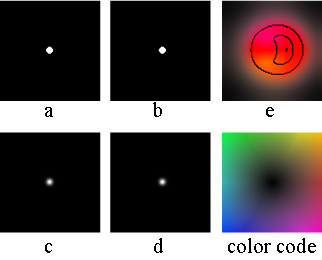
\includegraphics{./img/ex_dot_convol.png}
 \caption{Moving point source simulating a fluorescent signal in a confocal 
          microscopy image, and its corresponding CLG-OF vector field.
          \textbf{a,b}: first and second time frames. \textbf{c,d}: PSF-convolved 
          images from a,b according to the theoretical confocal microscope PSF. 
          \textbf{e}: CLG-OF vector field computed with $\alpha = 200$, $\rho = 5$, 
          $\sigma = 0$, and 500 iterations. The OF vector directions are colored 
          according to the color code. Pixel size corresponds to 107nm in 
          $x$ and $y$. The displacement of the signal between the two frames is 
          3 pixels (321nm).}
 \label{fig:ex1}
\end{figure}



\begin{figure}
 \centering
 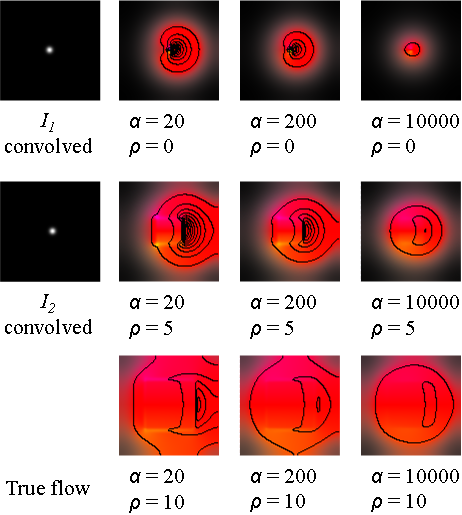
\includegraphics{./img/ex_dot.png}
 \caption{Different parameter values for CLG-OF and their corresponding OF fields 
          for the baboon image, with an horizontal displacement of one pixel.
          \textbf{$I_1$,$I_2$} are the input time frames.}
 \label{fig:ex2}
\end{figure}

\begin{figure}
 \centering
 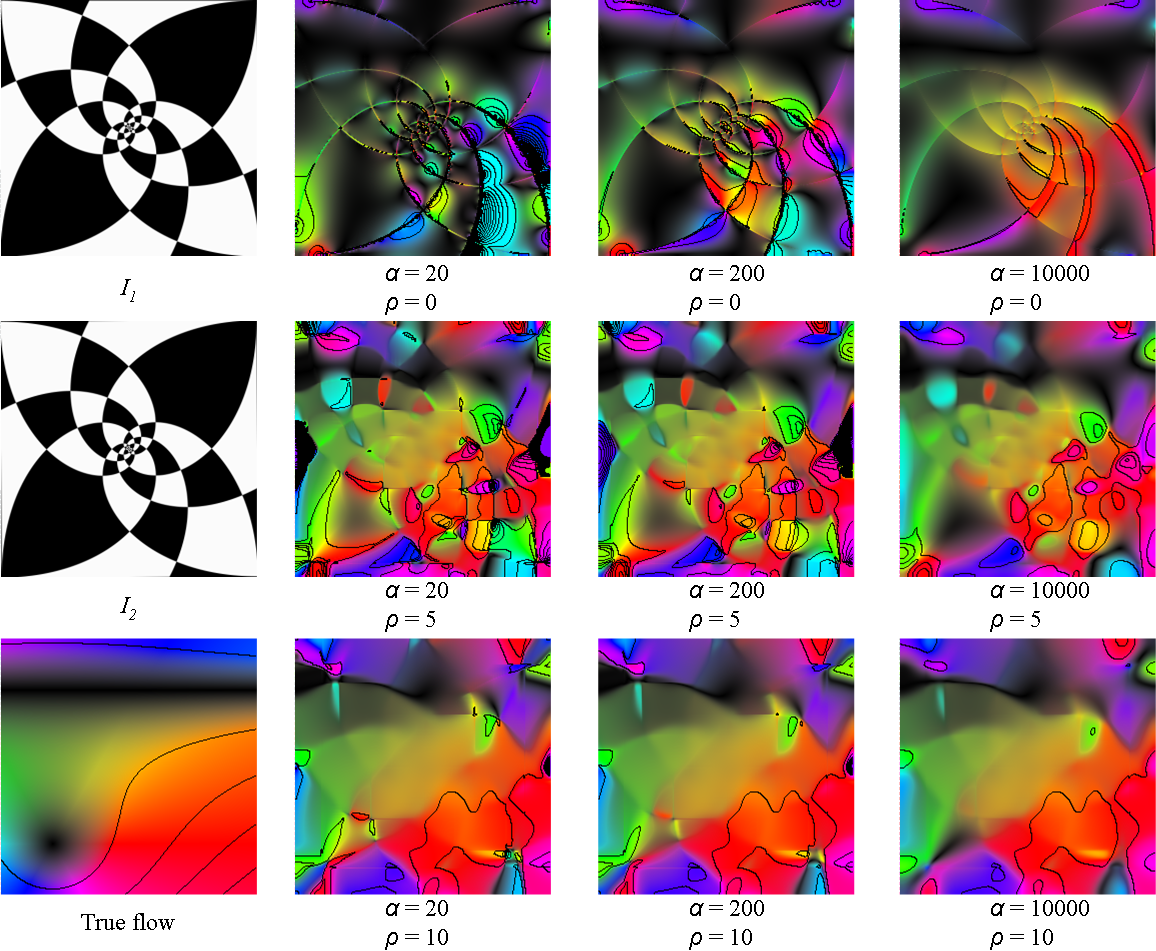
\includegraphics[width=1.00\textwidth]{./img/ex_spiral_hom.png}
 \caption{Different parameter values for CLG-OF and their corresponding OF fields 
          for the spiral image, with the homography transformation.
          \textbf{$I_1$,$I_2$} are the input time frames.}
 \label{fig:ex3}
\end{figure}


\begin{figure}
 \centering
 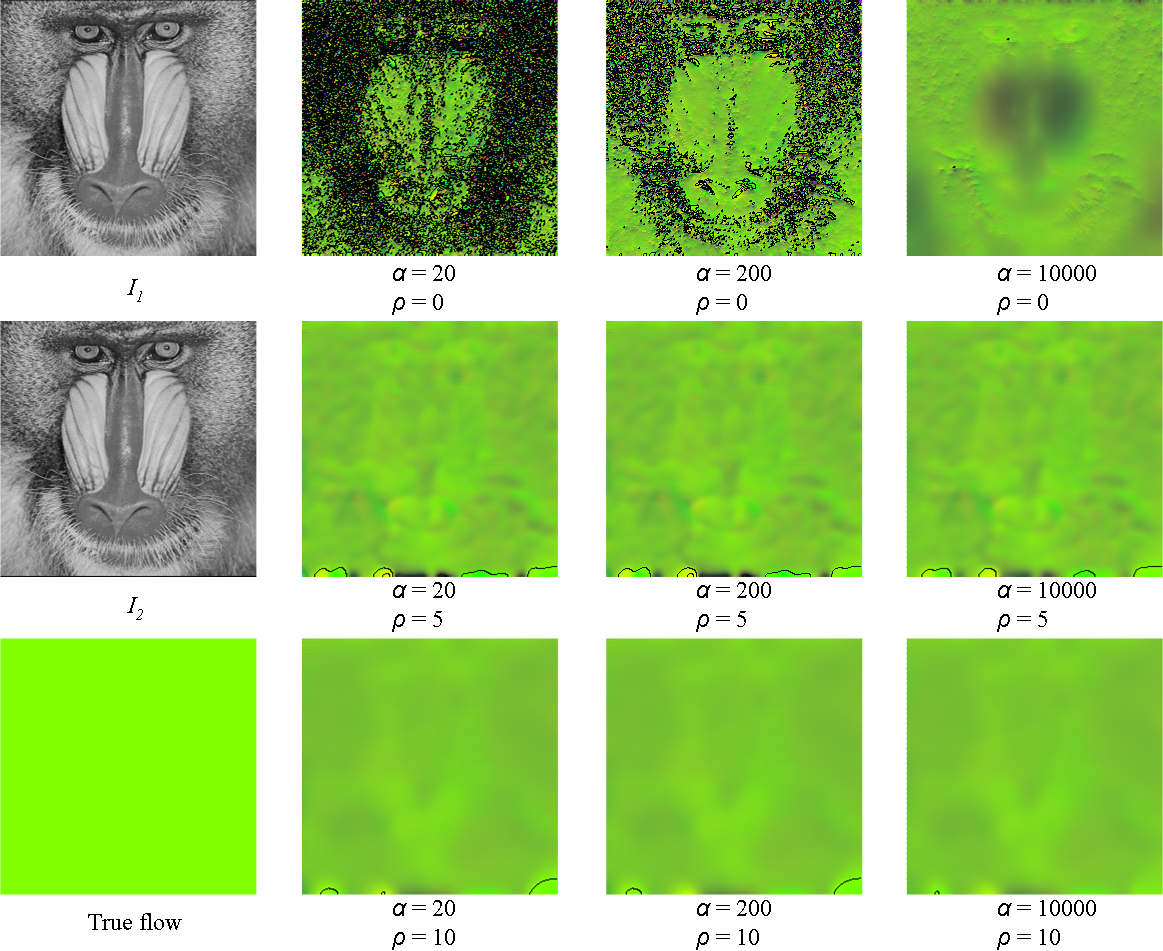
\includegraphics[width=1.00\textwidth]{./img/ex_baboon_one.png}
 \caption{Different parameter values for CLG-OF and their corresponding OF fields 
          for the baboon image, with an horizontal displacement of one pixel.
          \textbf{$I_1$,$I_2$} are the input time frames.}
 \label{fig:ex4}
\end{figure}


\begin{figure}
 \centering
 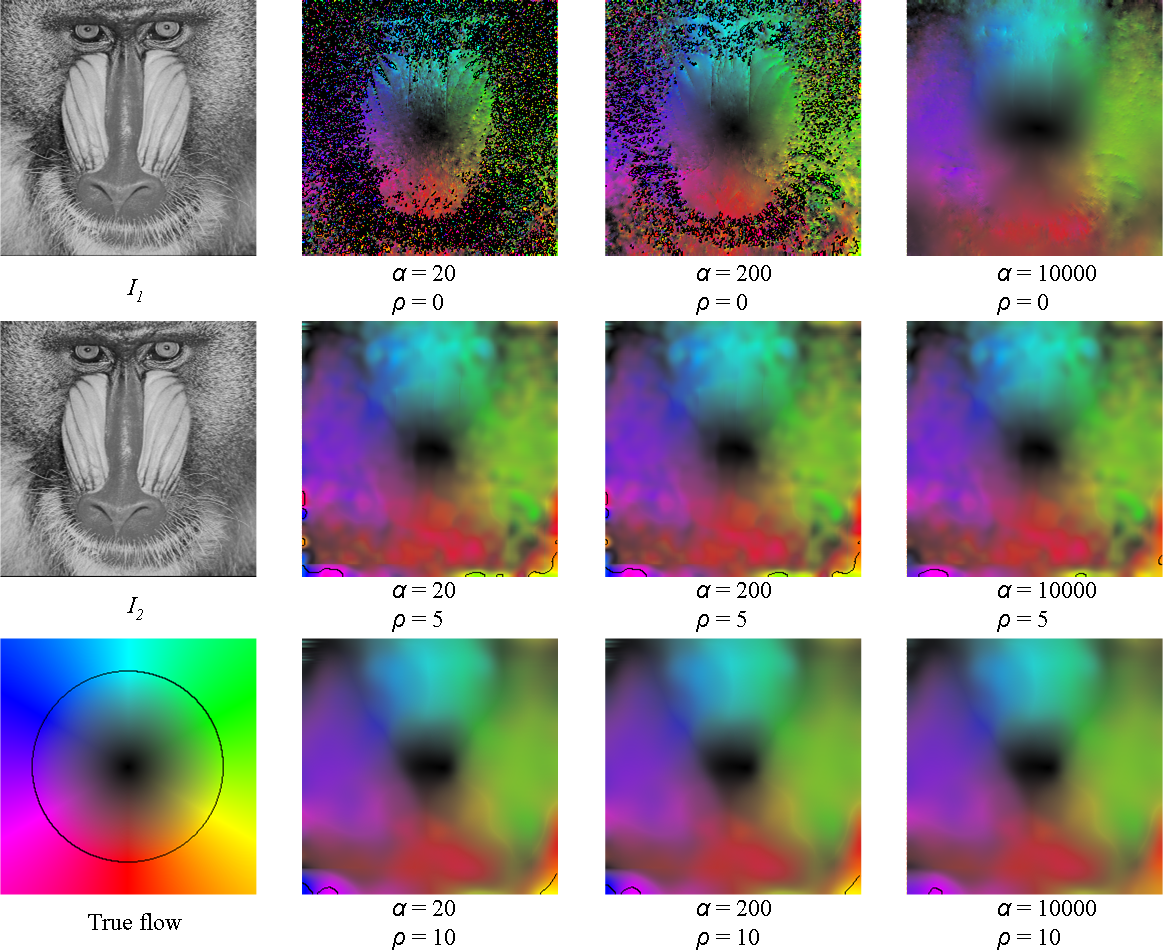
\includegraphics[width=1.00\textwidth]{./img/ex_baboon_rot.png}
 \caption{Different parameter values for CLG-OF and their corresponding OF fields 
          for the baboon rotation images.
          \textbf{a,b}: first and second time frames. \textbf{c-g}: CLG-OF fields 
          computed for different values of $\alpha$ and $\rho$.}
 \label{fig:ex5}
\end{figure}


\bibliographystyle{plain} %Styles: plain / apalike / amsalpha / ...
\bibliography{clgReferences}

\end{document}
